% Models overview: non-reasoning families x parameter buckets, with the
% reasoning-trained Qwen3 8B set apart as a boundary case.
% Requires only: \usepackage{tikz}\usepackage{graphicx}  (no extra tikzlibraries)
% Single-column safe: wrapped in \resizebox{\columnwidth}{!}{...}.
% NOTE: this is a floating figure. Do NOT place it inside a minipage/parbox
%       (that triggers "Not in outer par mode" and the figure vanishes).
\definecolor{qwenF}{HTML}{D3E2F5}\definecolor{qwenE}{HTML}{2F6DB0}\definecolor{qwenT}{HTML}{1C4A7E}
\definecolor{gemF}{HTML}{D8ECD2}\definecolor{gemE}{HTML}{4A8A3F}\definecolor{gemT}{HTML}{2F5E29}
\definecolor{misF}{HTML}{F6E4C9}\definecolor{misE}{HTML}{C08A35}\definecolor{misT}{HTML}{8A6320}
\definecolor{q3F}{HTML}{E7E7E7}\definecolor{q3E}{HTML}{8A8A8A}\definecolor{q3T}{HTML}{555555}
\definecolor{bandC}{HTML}{F4F3EF}

\begin{figure}[t]
\centering
\resizebox{\columnwidth}{!}{%
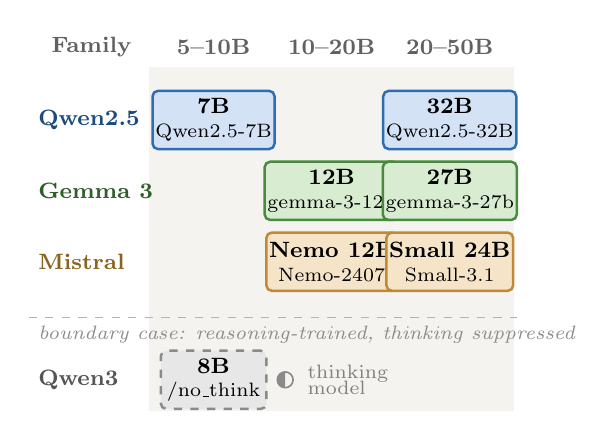
\begin{tikzpicture}[
  card/.style 2 args={draw=#1, fill=#2, line width=0.9pt, rounded corners=2pt,
                      minimum width=1.34cm, minimum height=0.74cm, align=center,
                      inner sep=1pt, font=\footnotesize},
  hdr/.style={font=\footnotesize\bfseries, text=black!62},
]
% parameter-bucket column bands (drawn first = behind)
\foreach \cx in {2.45, 3.95, 5.45}
  \fill[bandC] (\cx-0.82,0.55) rectangle (\cx+0.82,4.92);

% column headers
\node[hdr] at (0.9,5.18) {Family};
\node[hdr] at (2.45,5.18) {5--10B};
\node[hdr] at (3.95,5.18) {10--20B};
\node[hdr] at (5.45,5.18) {20--50B};

% --- non-reasoning families ---
\node[font=\footnotesize\bfseries, text=qwenT, anchor=west] at (0.10,4.25) {Qwen2.5};
\node[card={qwenE}{qwenF}] at (2.45,4.25) {\textbf{7B}\\[-1pt]{\scriptsize Qwen2.5-7B}};
\node[card={qwenE}{qwenF}] at (5.45,4.25) {\textbf{32B}\\[-1pt]{\scriptsize Qwen2.5-32B}};

\node[font=\footnotesize\bfseries, text=gemT, anchor=west] at (0.10,3.35) {Gemma 3};
\node[card={gemE}{gemF}] at (3.95,3.35) {\textbf{12B}\\[-1pt]{\scriptsize gemma-3-12b}};
\node[card={gemE}{gemF}] at (5.45,3.35) {\textbf{27B}\\[-1pt]{\scriptsize gemma-3-27b}};

\node[font=\footnotesize\bfseries, text=misT, anchor=west] at (0.10,2.45) {Mistral};
\node[card={misE}{misF}] at (3.95,2.45) {\textbf{Nemo 12B}\\[-1pt]{\scriptsize Nemo-2407}};
\node[card={misE}{misF}] at (5.45,2.45) {\textbf{Small 24B}\\[-1pt]{\scriptsize Small-3.1}};

% --- boundary-case divider + reasoning model ---
\draw[black!30, dashed, line width=0.6pt] (0.10,1.74) -- (6.30,1.74);
\node[font=\scriptsize\itshape, text=black!45, anchor=west] at (0.10,1.52)
  {boundary case: reasoning-trained, thinking suppressed};

\node[font=\footnotesize\bfseries, text=q3T, anchor=west] at (0.10,0.95) {Qwen3};
\node[card={q3E}{q3F}, dashed] at (2.45,0.95) {\textbf{8B}\\[-1pt]{\scriptsize /no\_think}};
% half-filled "thinking" mark + label
\begin{scope}[shift={(3.36,0.95)}]
  \draw[q3E, line width=0.6pt] (0,0) circle (0.10);
  \fill[q3E] (0,0.10) arc (90:270:0.10) -- cycle;
\end{scope}
\node[font=\scriptsize, text=black!50, anchor=west, align=left] at (3.52,0.95) {thinking\\[-2pt]model};
\end{tikzpicture}}
\caption{\textbf{Models.} Three families that were \emph{not} trained for
reasoning, so an inserted insight is informative rather than redundant. Each is
sampled at two sizes and crossed with parameter buckets (5--10B, 10--20B,
20--50B) to enable both intra-family (size) and inter-family comparisons.
Qwen3 8B with thinking disabled (\texttt{/no\_think}) is set apart as a boundary
case: reasoning-trained but reasoning-suppressed, treated as a contrast rather
than a clean non-reasoning model. It is also the one model that breaks the
ordering pattern (\S\ref{sec:h3}).}
\label{fig:models}
\end{figure}
